\documentclass[main.tex]{subfiles}

\begin{document}
\section{Dáta}

\subsection{Prieskumy volebných preferencií}
Na účely tohto projektu potrebujeme mať značnú históriu volebných prieskumov v jednotnom formáte. Budeme sa zaoberať voľbami v rokoch 2012, 2016, 2020 a 2023, čiže potrebujeme prieskumy z obdobia od januára 2010.
Nakoľko však agentúra FOCUS nezverejňuje s každým prieskumom jednotný .xlsx alebo .csv súbor a rovnako na svojej stranke nemá zverejnené všetky prieskumy, ktoré kedy vykonala, tak je táto úloha obzvlášť problematická.
Väčšina vykonaných prieskumov je však k dispozícií vo formáte .pdf v štýle reportu (Press release). Javí sa, že FOCUS pri týchto reportoch udržuje jednotný formát v priebehu rokov, čo využijeme na extrakciu dát z nich.

Súčasťou každého takéhoto .pdf súboru je aj samotný prieskum, napríklad:

\begin{center}
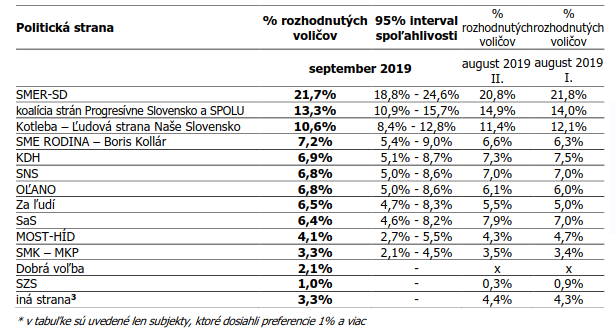
\includegraphics[width=0.7\textwidth]{figs/priklad-focus-prieskumu.png}
\end{center}

Automatizovaného sťahovanie z webu sme vykonali pomocou Python knižnice \href{https://github.com/SeleniumHQ/Selenium}{Selenium}, ktorá vie interagovať s webovým prehliadačom ako bežný používateľ. Pomocou iteratívneho odosielania query do prehliadača vo forme: "focus prieskum volby {month} {year}" + " filetype:pdf" sme stiahli prvý result vo forme .pdf súboru. Avšak ak v danom mesiaci nebol uskutočnený prieskum, resp. prvý nájdený .pdf súbor obsahoval niečo iné, stiahli sme zbytočný súbor. Takéto situácie sme museli následne ručne identifikovať a odstrániť. 

Nakoniec sa nám úspešne podarilo takýchto reportov získať 127. 

Ďalej sme tabuľky z reportov agentúry FOCUS automatizovane extrahovali na účel vytvorenia jednotného .csv súboru. Použili sme Python knižnicu \href{https://github.com/DS4SD/docling}{Docling}, pomocou ktorej sme prekonvertovali tabuľky z .pdf do pd.DataFrame, spojili a exportovali do jednotného \verb*|data/raw/polls/focus_polls.csv|.

Tento proces nebol úplne priamočiary. Názvy politických strán sa extrahovali veľmi nekonzistentne.
Takisto viaceré politické strany menili meno v priebehu rokov, takže bolo potrebné manuálne vytvoriť mapper, ktorý tieto názvy zjednotil. Ďalej bolo potreba niektoré záznamy aj manuálne opraviť, keďže strany s dlhším názvom (v reporte zabrali dva riadky tabuľky) sa duplikovali v našom extrahovanom datasete.

Prieskumy z obdobia od januára 2010 do novembra 2024, ktoré sme neboli schopní získať automatizovane, sme dopísali ručne. Agentúra Focus však nezverejňuje výsledky každý mesiac, čiže sme tieto údaje doplnili z iných agentúr. Vyskytlo sa však 10 mesiacov, kedy žiadna známa agnetúra prieskum nezverejnila. Tieto dáta sme lineárne interpolovali zo \enquote{susedných} mesiacov. Údaje o zdrojoch jednotlivých prieskumov sú v súbore \verb*|data/polls_agencies.csv|. Výsledné dáta z prieskumov sú v súbore \verb*|data/polls_data.csv|.

\subsubsection*{Rozdelenie prieskumov podľa volieb}

Pre neskoršie účely regresie a klasifikácie potrebujeme poznať výsledky jednotlivých volieb pre jednotlivé strany. Tieto údaje sme získali zo \href{https://volby.statistics.sk/}{Štatistického úradu Slovenskej republiky}, sú uložené v súbore \verb*|data/election_results.csv|. Takisto môže pri klasifkácii/predikovanii pomôcť údaj, či bola daná strana v konkrétnom volebnom období v koalícii/opozícii. Tieto údaje boli vyplnené ručne do súboru \verb*|data/elected_parties.csv|. K týmto dátam sme ešte pre každú stranu pridali jej politické preferencie z prieskumov 12 mesiacov pred voľbami, čo môžete nájsť v súbore \verb*|data/polls_by_election.csv|.

Tieto dáta chceme využiť v dizajne modelov, preto ich rozdelíme na trénovaciu a testovaciu sadu v pomere $4:1$. Treba však odfiltrovať dáta, ktoré sú podobné typu \enquote{volebný výsledok 0\%, všetkých 12 prieskumov pred voľbami okolo 0\%}, aby sme mohli pozorovať trendy a správanie, nie iba konštantnú nulu. Preto sú v trénovacom a testovacom datasete iba tie strany, ktoré počas 12-tich mesiacov pred konkrétnymi voľbami dosiahli aspoň raz hranicu 1.5\%, čo je polovica hranice na štátny príspevok za výsledok vo voľbách. Vo výsledku je teda v datasete \verb*|data/polls_by_election_train.csv| 50 dátových bodov, v \verb*|data/polls_by_election_test.csv| 13.

\subsection{Všeobecné štatistiky o štáte}

V modelovaní chceme zistiť, či interakcia hodnoty rôznych indikátorov o Slovenskej republike napríklad s účasťou v koalícii nezachytáva nejaké trendy. Preto sme z portálu \href{https://datacube.statistics.sk/}{DATAcube} získali dáta o nasledovných indikátoroch pre roky 2010 až 2023 (vymenované sú iba tie, ktoré sú použité v neskoršej analýze)

\begin{itemize}
	\item nezamestnanosť v percentách
	\item HDP na človeka v eurách
	\item riziko chudoby v percentách
	\item priemerný príjem v domácnosti v eurách za mesiac
	\item inflácia v percentách
	\item priemerná cena benzínu s oktánovým číslom 95 v eurách za liter
	\item výdavky na vedu a vzdelávane v eurách za rok
\end{itemize}

Tieto dáta sú uložené v súbore \verb*|data/general_data.csv|.

\subsection{Politický kompas}

Ako posledné sme chceli získať údaje o hodnotách a nastaveniach politických strán. Získali sme nasledovné údaje z \href{www.google.com}{\LARGE ZDROJ AKÝ?} pre politické subjekty Progresívne Slovensko, Smer SD, Hlas SD, Slovensko, SaS, KDH, Republika, SNS, Sme rodina, Maďarská aliancia a Demokrati:

\begin{itemize}
	\item liberalizmus-konzervativizmus: na škále od -1 do 1, kde -1 je najviac liberálny
	\item ľavica-pravica: na škále od -1 do 1, kde -1 je najviac ľavicový
	\item životné prostredie: na škále od -1 do 1, kde 1 značí najväčší možný dôraz na témy týkajúce sa životného prostredia
	\item integrácia v Európskej únii: na škále od -1 do 1, kde 1 značí najväčší možný dôraz na témy týkajúce sa integrácie do EÚ
	\item internacionalizmus a zahraničná politika: na škále od -1 do 1, kde 1 značí najväčší možný dôraz na témy týkajúce sa zahraničnej politiky a spolupráce so zahraničím
\end{itemize}

Tieto dáta sú uložené v súbore \verb*|data/political_compass_data.csv|.

\end{document}
